\chapter{Background}
\label{sec:state}

% Hier werden zwei wesentliche Aufgaben erledigt:

% 1. Der Leser muß alles beigebracht bekommen, was er zum Verständnis
% der späteren Kapitel braucht. Insbesondere sind in unserem Fach die
% Systemvoraussetzungen zu klären, die man später benutzt. Zulässig ist
% auch, daß man hier auf Tutorials oder Ähnliches verweist, die hier auf
% dem Netz zugänglich sind.

% 2. Es muß klar werden, was anderswo zu diesem Problem gearbeitet
% wird. Insbesondere sollen natürlich die Lücken der anderen klar
% werden. Warum ist die eigene Arbeit, der eigene Ansatz wichtig, um
% hier den Stand der Technik weiterzubringen? Dieses Kapitel wird von
% vielen Lesern übergangen (nicht aber vom Gutachter ;-), auch später
% bei Veröffentlichungen ist "Related Work" eine wichtige Sache.

% Viele Leser stellen dann später fest, daß sie einige der Grundlagen
% doch brauchen und blättern zurück. Deshalb ist es gut,
% Rückwärtsverweise in späteren Kapiteln zu haben, und zwar so, daß man
% die Abschnitte, auf die verwiesen wird, auch für sich lesen
% kann. Diese Kapitel kann relativ lang werden, je größer der Kontext
% der Arbeit, desto länger. Es lohnt sich auch! Den Text kann man unter
% Umständen wiederverwenden, indem man ihn als "Tutorial" zu einem
% Gebiet auch dem Netz zugänglich macht.

% Dadurch gewinnt man manchmal wertvolle Hinweise von Kollegen. Dieses
% Kapitel wird in der Regel zuerst geschrieben und ist das Einfachste
% (oder das Schwerste weil erste).

% Background Warum ist das Thema wichtig?
% Was ist das Smart Grid -> mit Background verknüpfen
% Vor, Nachteile vom Smart Grid?
% Was sind Smart Meter
% Warum sind Smart Meter Privacy relevant?
% DC-Netze einführen
% Related Work: Welche andere Verfahren gibt es?
% Vllt erklärung regeln vom BSI

The following section explains the key components of the smart grid, the structural changes as well as the occurring challenges that need to be solved. The overview provides the fundamental understanding of this work. Because this thesis requires a basic understanding of the German smart grid, the stakeholders and their interests in the smart grid are expounded. In addition, the technical guideline from the \gls{BSI}\footnote[1]{BSI - Bundesamt für Sicherheit in der Informationstechnik(eng. Federal Office for Information Security)} is introduced because it defines a first security-relevant standard required for all smart meters in the German smart grid. Moreover, this chapter discusses the current state of research and the solutions which are discussed in the scientific community.\\

\section{Smart Grid}
The original energy network was mainly considered as a transmission system to send electricity from the generators via an elongated network of cables and transformers to the consumers.% vllt hier noch schreiben, dass es erneuerbare Energien wegen der Klimakriese gibt
The distribution from the traditional few electricity producers (e.g. nuclear power plants, coal-fired power plants), which were responsible for a large part of the electricity generation, is changing to a rising number of smaller producers (e.g. wind turbines), due to the increased integration of renewable energies. %However, renewable power generation is often dependent on external environmental influences. Therefore, smart meters have been widely introduced in households to ensure that the smart grid is stable despite fluctuations in power generation.
But, renewable power generation is often depending on external environmental factors. In order to maintain a stable grid, smart meters are used to increase the overall grid quality through regular communication of status information and power consumption. Smart meters enable the electricity provider to receive the electricity consumption of a household every 15 minutes. This offers the possibility to access the current electricity demand from the consumers more easily. Previously, the current electricity demand was simulated from load forecasting models. If the demand should increase spontaneously, peaker plants, mainly consisting of gas-fired power plants, would be turned on to quickly meet the demand. This is costly and environmentally unfriendly. 
Since then, structural changes were made in order to optimize the energy grid and make it more intelligent by exchanging information in near-real-time. This allows the demand to match with the available supply. The fundamental component of the smart grid are the smart meters which will be discussed more detailed in the following paragraph \cite{fan2012smart}\cite{zeadally2013towards}.\\
\\
\textbf{Smart Meter}
\\
\\
Smart meters are the essential component in a smart grid. It is an electricity meter which has an interface to the Internet. Beside the metering of the power consumption for electricity provider the additional functions of a smart meter are to provide a two-way communication between the electricity grid participants and the smart meter. The participants receive the status data from the smart meter and process it further.
The extended transmission of information between smart meters and electricity grid participants via the Internet is also called Advanced Metering Infrastructure \gls{AMI}. The resulting communication between the components improves the quality of the power grid and makes it possible to offer new services. For example, detecting power outages used to be depending on customer calls whereas nowadays the grid operator can do that itself.\\
Another new feature is a detailed monitoring of power flows at the smart meter, instead of only measuring it up to substations like before. Moreover, the advanced functions enable electricity network operators to quickly detect changes in consumption behavior and react to them without having to use costly and environmentally unfriendly peaker plants. Depending on the setting, smart meters can send electricity consumption to the electricity provider at least every 15 minutes. Additionally, in combination with the consumption of all users and the current electricity supply, real-time pricing becomes possible. Not only the customer can be offered a better electricity contract, the smart meters no longer have to be read out at home by a technician from the electricity provider. As a result billing becomes easier for customers and electricity providers. Furthermore, customers can also check their current electricity consumption via the interfaces provided by the smart meter in order to analyze their own behavior and to reduce their consumption \cite{finster2014privacy}. 
%Thus, the end user can analyze his own consumption behavior in order to reduce his own electricity consumption.
\section{Smart Meter Privacy}
The main advantage of the smart grid is the advanced communication between the consumers smart meter and the energy suppliers. The messages every 15 minutes from the electricity meter provide the electricity supplier with a regular update on the status of the electricity grid and there is no longer any need to rely on forecasting models based on data from the past. However, sending user information in such a short period of time allows new methods to be used to create accurate behavioral analyses in an individual home. Sending private electricity consumption data is therefore very sensitive information and has to be protected. This is not an easy task, because on the one hand the electricity consumption must be protected and anonymized, and on the other hand the billing and costs must be clearly assignable to a person. The two problems are referred to as Metering for Billing and Metering for Operations. At first it is described how simple behavioral analyses are generated by electricity consumption. Subsequently, solutions to Metering for Billing and Metering for Operations will be presented, that have been discussed in the scientific community so far \cite{finster2014privacy}. \begin{figure}[htbp!]
  \centering
  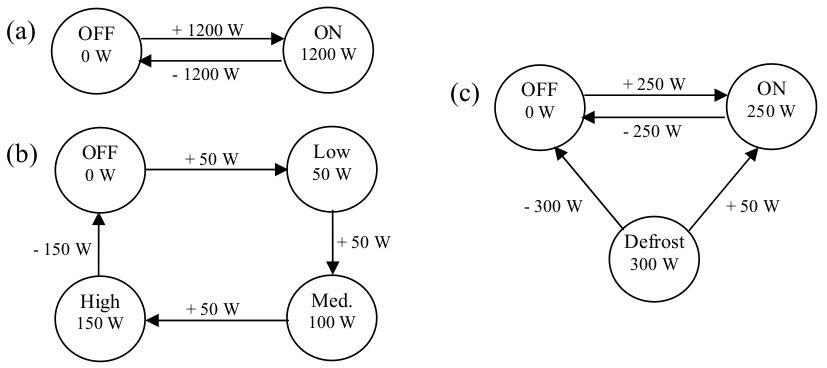
\includegraphics[width=0.9\textwidth]{images/Appliance_Model.png}
  \caption[Appliance Model]{Sample Appliances after performing step 3. (a) represents a toaster that has 2 states. (b) is a lamp that has 3 different brightness levels. (c) shows a refrigerator with defrost mode \cite{quinn2009privacy}.}
  \label{fig:Appliance_Model}
\end{figure}
\subsection{Non-intrusive load monitoring} 
\label{subsec:NILM_sec}
Interpreting electricity consumption with the intent of identifying devices at home is called non-intrusive load monitoring \gls{NILM}. George Hart and Fred Schweppe were the first to develop non-intrusive load monitors in 1985 and connected them to electricity meters \cite{hart1989residential}. They were able to record the current electricity consumption up to every 5 seconds. They developed a five step procedure to detect household appliances that can be explained like this.
\begin{enumerate}
\item Edge Detection:\\
First, the intercepted electricity consumption is stored. Second, a search in the stored data for strongly rising or strongly falling edges is performed. These edges indicate that a device may have been switched on or off at one specific moment.
\item Cluster Analysis:\\ 
The stored events of steeply rising or steeply falling edges are visualized in a graph with the following characteristics. Each event is ordered according to how much electricity was consumed or how much electricity was 	``released'' from the device (e.g. when it was switched off). This causes similar events to be recognizable as clusters in the diagram.
Essentially, a cluster analysis is then applied to the diagram and each found cluster represents a household appliance.
\item Appliance Model Construction\\
Since different household appliances have been determined by the clusters, appliance models can now be constructed. In this step, different states in which an appliance can be in, are found based on the different electricity consumption. An example of how the result of a appliance model looks like can be seen in Figure \ref{fig:Appliance_Model}.
\item Behavior Analysis:\\
Once the majority of the household appliances have been identified, the behaviors of people in the household can be analyzed. In real time, it is possible to track the use of devices, since individual signals can be identified as they occur and do not need to be reconstructed anymore.
At this point, several approaches can be taken to provide behavioral analysis. A common approach is to track how long a device has been in use and create statistics on how each device has been used. A daily analysis can be viewed in Figure \ref{fig:Nilm}.
\item Appliance Saving:\\
The last approach is to name the household appliances found (washing machine, etc.) and store them in a database. So that in the case of a further household analysis, it is possible to fall back on appliances that have already been found.
\end{enumerate}
The founder of \gls{NILM} G. W. Hart himself said in 1989: ``Specifically, I recommend that legal restrictions be enacted or clarified so that electric power usage is considered as private as any phone conversation.''(Residential Energy Monitoring)
Through \gls{NILM}, simple observations can be made without analyzing the household behavior for a longer time. For example, it can be noticed when no one is at home because all lamps are turned off. It can also be quickly assumed that the house inhabitants are on vacation, if the electricity consumption is lower than usual. For burglars, this information would be particularly useful, as they would have no problem knowing when is a suitable time to break in.
\begin{figure}[tbp]
  \centering
  \includegraphics[width=1\textwidth]{images/nilm.png}
  \caption[Detected NILM Appliances]{The electricity consumption of a household with drawn household appliances detected by \gls{NILM} \cite{quinn2009privacy}.}
  \label{fig:Nilm}
\end{figure}
\\
\\
\textbf{High Resolution Analysis}
\\
\\
Since then, research in the field of intrusive monitoring has continued. It was investigated both how much information can be extracted from the household through electricity consumption when electricity consumption was measured particularly frequently. Furthermore, it was investigated whether assumptions can be made about the behavior in the household even at low resolution.
For example, in the paper \cite{greveler2012multimedia}, the movie being watched could be determined by the electricity consumption of an LCD television. TV electricity consumption is strongly influenced by blacklighting activities. Each movie has a unique brightness signature, which was exploited to make a statement about the film being viewed.\\
%In the paper, the power consumption of the TV was measured every 2 seconds and after 5 minutes analysis of the consumption, the content of the program could be determined with high probability. For this purpose, a Power Consumption Prediction Function was trained to estimate the power consumption of the TV based on the brightness of movie sequences. The input of the prediction function is 5 minute sequences of a movie and the output is the possible power consumption of the TV.
In the paper, the electricity consumption of the TV was measured and stored every 2 seconds. After 5 minutes of analyzing the consumption, the content of the program could be determined with high probability. For this purpose, a Power Consumption Prediction Function was trained to estimate the power consumption of the TV based on the brightness of movie sequences. 
%The main goal is, that the Power Consumption Prediction Function can correctly guess/estimate the electricity consumption of the analyzed TV. If the estimation approximates the real stored power consumption of a stored movie, the movie is chosen by the function.
The input of the prediction function is 5 minute sequences of a movie and the output is the possible power consumption of the TV. 
In order to recognize a movie, the possible power consumption of the TV by the prediction function is stored over the 5 minute movie sequences. If the same 5 minute sequences are running on a TV, the power consumption can be compared with the prediction of the function by a correlation coefficient. For multiple matches with a correlation coefficient higher than 0.85, an additional optimization algorithm is applied to estimate the movie. Later, the paper also showed that the power consumption could be used to identify which TV channel was being watched. In the figure \ref{fig:tv} the result of the estimation of the prediction function is shown in green and in red the actual power consumption of a LCD TV for the same movie sequence can be seen. 
\begin{figure}[tbp]
  \centering
  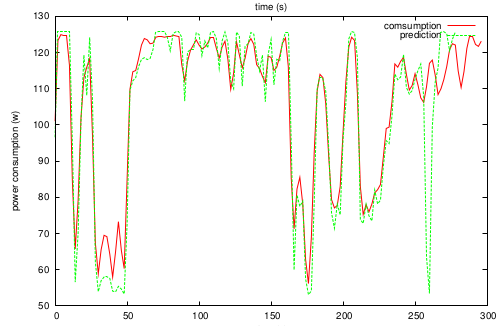
\includegraphics[width=1\textwidth]{images/Fernseher.png}
  \caption[Estimated power consumption of a TV]{The power consumption of a TV in green vs. the estimated power consumption of the TV using the prediction function in red \cite{greveler2012multimedia}.}
  \label{fig:tv}
\end{figure}
\\
\\
\textbf{Low Resolution Analysis}
\label{subsec:low_reso}
\\
\\Another approach is to work backwards from large data sets to obtain detailed information from aggregated electricity consumption. The \gls{NILM} procedure attempted to have household appliances detected from individual households and then behavioral analyses could be generated from the household appliances. A common approach with low-resolution electricity data is to identify the numerous factors that influence total electricity consumption and to filter them out \cite{quinn2009privacy}.
But with low resolution methods, a variety of approaches are being pursued.
For example in \cite{prudenzi2002neuron} an artificial neural network was trained to identify household appliances from electricity consumption. The electricity consumption was measured only every 15 minutes. The same time interval is used by \gls{SMGW}s as well. With the low resolution, only the household appliances that have a high overall impact on electricity consumption, such as refrigerators, were considered. A total of 10 different household appliances were attempted to be correctly identified from the electricity consumption. With the final trained ANN, an accuracy of 90\% was found.
\\%nochmal machen
In another work \cite{kolter2010energy}, the electricity consumption of appliances was measured only every hour. The experiment tried to disaggregate a aggregated electricity consumption with Discriminative Sparse Coding. The experiment was conducted as follows. First, the disaggregation algorithm was trained with electricity consumption of houses from a large data set. Then, the trained algorithm was applied to the aggregated electricity consumption of two houses. The algorithm was expected to determine up to 52 individual household appliances from the electricity consumption. The results in the paper showed that the disaggregation algorithm with Discriminative Sparse Coding was up to 55.05\% correct in its decisions.\footnote[2]{Considering the fact that the time interval is so small and 52 different household appliances were considered, the accuracy of 50\% is extraordinarily good. If the algorithm would only guess, the accuracy would be at 1.9\%.}

\section{Related Work}
After \gls{NILM} was discovered, the scientific community started to look for possible solutions to technically prevent the analysis of electricity consumption. In this chapter, the different approaches in Metering for Operations and Metering for Billing are presented. Although in this thesis only a solution of Metering for Operations is of importance, for completeness the solutions for Metering for Billing are introduced as well.
\subsection{Metering for Operations}
\label{subsec:Meter_for_Op}
\\
The paragraph deals with solutions for Metering for Operations, which have been discussed in other scientific works so far. At Metering for Operations, there is currently no established consensus on a solution. Various technical proposals have already been published in scientific papers, but there is a lack of standardized criteria and often different conditions are set for the power grid. One reason for this could be the different realization of smart grids in different countries. In the following, the various approaches are divided into categories and propounded conceptually.\\
\\
\textbf{Anonymization or Pseudonymization
Without Aggregation}
\\
\\
This approach describes the removal of smart information that allows identification towards the electricity provider. Identifiable information can also be replaced by pseudonyms. Solutions with trusted third parties \gls{TTP} are often used in this case. A \gls{TTP} usually acts as an intermediary between the customer and the electricity provider. The \gls{TTP} must be acknowledged by all participants and take a neutral position. In practice, however, this is difficult to achieve because the \gls{TTP} is often hired as a service provider by the electricity provider and is therefore also paid by the provider.\\
In the paper "A privacy-preserving Concept for Smart Grids" by Petrlic \cite{petrlic2010privacy}, a \gls{TTP} is used as an intermediary. In the procedure, a smart meter communicates with a \gls{TTP}. Certificates formed with a public key infrastructure are used to verify and validate information flows from smart meters at the \gls{TTP}. As soon as the \gls{TTP} has checked the correctness of the smart meter information, it can pseudonomize all necessary information. Only then is the further processed anonymized information forwarded to the electricity provider by the \gls{TTP} in encrypted form. This means that the electricity provider cannot assign individual electricity consumption to its customers. With this procedure, smart meters can be anonymized. 
However, if it is possible for an attacker to record the data traffic between the smart meter and the \gls{TTP}, then the attacker could forward the time stamps and smart meter identification to the electricity provider. Using these two pieces of information, the electricity provider could at least gain some insight, since it would be possible to match when information is sent to the \gls{TTP} and when it is received by electricity provider\cite{finster2014privacy}. \\
\\
\textbf{Aggregation with Trusted Third Parties}
\\
\\
In the attack just described, the electricity provider tries to link two events. One is the arrival of the message at the \gls{TTP} and the other is the arrival of the message at the provider itself. One way to prevent this attack is aggregation. In this case, the smart meter sends its electricity consumption to the \gls{TTP}. Certificates are additionally sent from the smart meter so that the \gls{TTP} can check the information for correctness and authenticity. Instead of forwarding the information to the electricity provider, the \gls{TTP} waits until all smart meters have sent their data for which the \gls{TTP} is responsible. This data is all added up and a message is sent from the \gls{TTP} to the electricity provider with the total electricity consumption of all smart meters. From the aggregated value, it is not possible to extract an individual smart meter's electricity consumption, which is why the electricity provider cannot filter out information about individual customers \cite{bohli2010privacy}.\\
Homomorphic encryption approaches also fall into this category. Homomorphic encryption algorithms allow simple operations such as addition and multiplication to be performed on the encrypted messages.  In some homomorphic encryption schemes, only addition or multiplication is supported. These algorithms are then called partial homomorphic encryption.
There are also bihomorphic encryption approaches. Here not only the operations on the ciphertexts are homomorphic, but also the operations on the keys. This means that if a plaintext $a$ is encrypted with the key $x$ and a plaintext $b$ is encrypted with the key $z$, that one can decrypt the ciphertexts $enc(a+b)$ with the keys $x+z$. A bihomomorphic encryption approach with \gls{TTP} has been proposed by Vetter et al\cite{vetter2012homomorphic}. In this case, the \gls{TTP} acts as the key authority. This means that it creates all cryptographic keys and forwards them to the smart meters, which are used for further communication with a central storage. The smart meter encrypts its data and sends it to the central storage. The central storage also saves the incoming data in encrypted form, so that no unencrypted data is stored. In addition, the central storage has no access to the keys and thus has no way to decrypt the information or access meaningful data.\\
Therefore, the central repository has to be trusted only in terms of functionality. If an electricity provider wants to know the electricity consumption of its customers, it makes a request to the central repository, which sends the aggregated encrypted data to the electricity provider. In order for the electricity provider to decrypt the data, the key authority has to release the correct keys. Moreover, it is impossible for the electricity provider to query the value of just one smart meter. This is because the key authority can only issue keys that can decrypt aggregated totals. It is guaranteed by the homomorphic encryption method which is used. The advantage of using the approach by Vetter et al. is that the different functionalities, namely storage of data and key acquisition for confidentiality and authenticity are realized from different participants.
\\
\\
\textbf{Aggregation Without a Trusted Third Party}
\label{subsec:aggegration_without_ttp}
\\
\\
The solution proposed in this thesis is also one of the methods that aggregates without a \gls{TTP}. The advantage of this approach is that no one has to trust a \gls{TTP}. In general, one has to ask the questions who aggregates the data and who generates the keys. In addition, a common problem to consider is, how the procedure deals with a few participants. \\
In the solution of Mármol et al. \cite{marmol2012not} again a bihomomorphic encryption method is proposed. The approach of Mármol has already been discussed and implemented in a master thesis at this chair\cite{Anna}. As a reminder, bihomorphic encryption algorithms can perform simple operations such as addition on both the ciphertext and the keys. This property is exploited in the presented method of Mármol. Since it aggregates the keys and not the electricity consumptions as before. Furthermore, it does not matter which bihomomorphic encryption method is used, as long as all smart meters agree on one method. A key is generated from every smart meter in the power grid. Afterwards, the generated key is used to encrypt the electricity consumption and the encrypted result is sent to the network operator. The transmission channel to the network operator is chosen in such a way that the identity of the smart meter remains unknown. This prevents the smart meter from exposing itself during communication with the operator. Groups are formed among smart meters and a smart meter aggregator is randomly selected in each group. All smart meters send their keys to this aggregator. Subsequently, the keys are summed up at the aggregator and sent to the network operator. The network operator receives a single key and with this key it can only decrypt the messages from one smart meter group. Additionally, the operator has to add up all the messages and only then it will be possible to decrypt the messages. There is a chance that the aggregator cooperates with the network operator. The aggregator would then be able to send individual keys from smart meters to the operator. While the operator would not be able to match the key to any message, by brute force it could decrypt all messages with that key and see which decrypted message has meaningful content. To prevent this attack, an additional measure is taken. All smart meters in a group organize themselves topologically in a ring structure. In this ring structure, all smart meters cooperate with each other and change their keys every round in such a way that the individual key of a smart meter changes, but not the summed key of all smart meters. Even if the aggregator forwards the keys to the network operator, they would no longer be valid in the following round. A disadvantage of this procedure is that if a smart meter leaves the group, then a new aggregated key must be formed and the operations are quite computationally expensive.\\
\\
\textbf{Battery Solutions}
\\
\\
The battery approach describes a household with a connected battery that is charged, e.g. by grid purchase or by photovoltaic panels. The goal of the approach is that the battery feeds energy into the household in such a way that the grid operator can no longer detect private information based on the electricity consumption. \\
\begin{figure}[tbp]
  \centering
  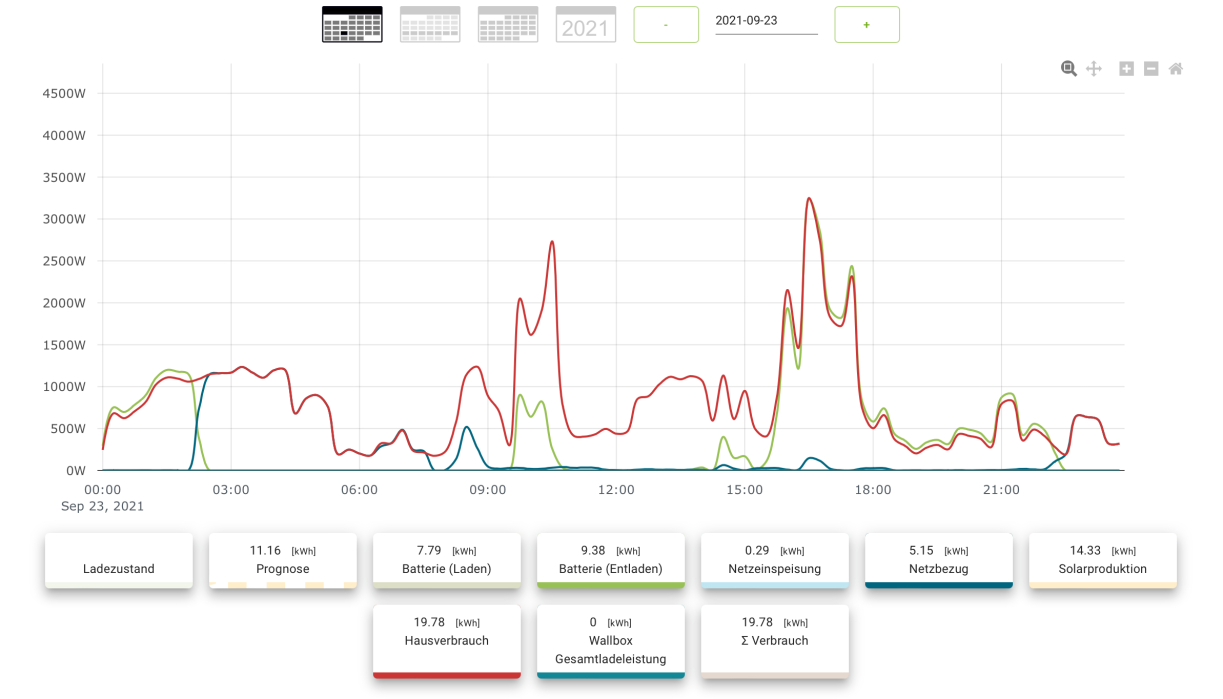
\includegraphics[width=1\textwidth]{images/Battery4.png}
  \caption[Battery Consumption Figure]{The electricity consumption of a household during the day (red) with battery (green) and the electricity consumption that the electricity provider can access (blue).}
  \label{fig:Battery}
\end{figure} Figure \ref{fig:Battery} shows the electricity consumption of a private household with a connected battery that is charged via solar panels. The red line shows the electricity consumption of the household. The green line shows when the battery is discharged (when the battery is feeding power to the household). The blue line is the electricity consumption that the electricity provider can see. As pictured in the figure when the battery is discharged, the electricity provider cannot detect any electricity consumption from the household. In other cases, the electricity provider notices that electricity is being consumed, but it is much less than the actual electricity consumption because the battery of the house offsets some of the electricity consumption. In other words, if a household is connected to a battery, the electricity provider cannot make correct statements about the behavior of the people in the household. \\
An algorithm for batteries was proposed in \cite{mclaughlin2011protecting}. This method uses an algorithm that can control the battery to produce a constant characteristic curve in consumption. The algorithm targets a static and fixed current consumption. The target consumption is calculated differently by the algorithm depending on the house consumption and battery capacity. If the electricity consumption is below the consumption set by the algorithm, then the battery is charged with the difference from the target consumption. If the electricity consumption is above the target consumption set by the algorithm, the battery is discharged with the difference from the target consumption. If the consumption is significantly higher, so that the battery can no longer absorb the additional consumption, then it is switched to recovery mode. In recovery mode, the target consumption is temporarily increased, so that the battery can charge on the side, even though the house is currently consuming a lot of electricity. If the recovery mode can be switched off, then a new target consumption is calculated based on the new data. It is important to remember that this method does not anonymize electricity consumption, so it is even more important to measure how much information can still be extracted from electricity consumption. There are the following metrics to calculate how much privacy is gained by the algorithm.
\begin{enumerate}
\label{subsec:information_gain}
\item Relative Entropy:\\
Relative entropy\footnote[3]{Relative entropy is often referred in literature as Information Gain or Kullback-Leibler divergence.} is used to compare two sources of information. In this case it would be the electricity consumption with the algorithm and the electricity consumption without the algorithm. These two loads form a stochastic process and can then be analyzed with the calculated relative entropy \cite{kalogridis2011affordable}. The relative entropy is defined as follows:\\
\begin{equation}
D(P\|Q) = KL(P, Q)= \sum_{x \in X} P(x) \cdot \log {P(x) \over Q(x)}
\end{equation}
\clearpage
\item Cluster Classification:\\
The cluster classification has already been explained for the \gls{NILM} method and described in this thesis at \ref{subsec:NILM_sec}. Cluster Classification is well known as a machine learning approach, but it can also be used as a metric to evaluate privacy. Here one would perform a cluster analysis with the battery method and once without. Then one looks at the number of clusters in both measurements and if fewer clusters are found with the battery method, then this is considered a privacy gain \cite{kalogridis2010privacy}.
\item Regression Analysis:\\
In the regression analysis, first a cross-correlation and afterwards a simple linear regression is performed. More precisely, both electricity consumptions are "superimposed" at the point of their maximum cross-correlation. Subsequently, a linear regression is performed and the privacy is evaluated on the basis of the quality of the predictor \cite{mclaughlin2011protecting}.
\end{enumerate}
\\
\\
\textbf{Drawbacks}
\\
\\
Although various approaches to solving Metering for Operations are discussed, the following drawbacks must also be considered.
\begin{enumerate}
\item Pseudonymization:\\
Pseudonymization does not provide protection against the attacks described in \ref{subsec:NILM_sec}. The only thing pseudonyms protect is the identification of the \gls{SMGW}. Once it is possible to assign the pseudonym to a customer, the pseudonym becomes invalid and the electricity consumption can be uniquely assigned to a customer. 

\item Aggregation with Trusted Third Parties\\
The approach of \gls{TTP}s is difficult to realize in the smart grid scenario. This is because the question of the neutrality of the \gls{TTP} remains open. The service of the \gls{TTP} is not free and it remains unclear which entity in the system will pay for the \gls{TTP}. If the customer were to bear the costs, then the electricity provider could question the neutrality of the \gls{TTP}. However, it is much more likely that the electricity provider will pay for the \gls{TTP}s service. In this case, the neutrality of the \gls{TTP} would be open to doubt by the customer, since the \gls{TTP} could be dependent on payments from the electricity provider.

\item Battery Approaches:\\
Battery methods are a good way to mask actual electricity consumption. However, it is also a physical device that needs to be installed in the home and is costly at the same time. Widespread installation of batteries on a large scale is therefore unlikely in the next few years, as not every household has the funds for this investment.

\item Aggregation without Trusted Third Parties:\\
A disadvantage of Aggregation without \gls{TTP}s procedures is their hire complexity at a conceptual level. In addition, many Aggregation without \gls{TTP} approaches involve homomorphic encryption schemes that are very computationally intensive. Nevertheless, the author believes that this category is the most appropriate for protecting client anonymity, because there is no need to rely on \gls{TTP} or invest a lot of money as in the battery approaches.
%vllt sowas wie, dass die verfahren etwas komplexer sind, da eine mögliche entität wegfällt(ttp),die aufgaben übernehmen könnte und die nun durch das verfahren aufgefangen werden muss. Trotz der Komplexität, können die verfahren allerdings performant sein. die verfahren müssen nur fein abgestimmt werden. Das ist der grund, weshalb 
\end{enumerate}
%dann sowas sagen wie, für jedes verfahren gibt es vor und nachteile. und das es der grund ist, weshalb noch keinen einheitlichen consens der umsetzung gibt.
\subsection{Metering for Billing}
In order to fully protect the privacy of a household, metering for billing procedures must also be applied. Otherwise, conclusions about electricity consumption may be drawn from the billing. A simple solution would be to increase the frequency of the billing period. But at the same time it is also in the interest of the customer to buy electricity as cheaply as possible and the customer can be offered better electricity contracts if the billing period is shorter. In addition, it cannot be guaranteed that the customer's privacy is not violated in more complex electricity contracts by other features, even if a higher billing period is used. %In the following paragraph, different methods are explained that solve the problem for metering for billing. 
This master thesis focuses mainly on the metering for operations problem. 
By implementing Trusted Platform Modules \gls{TPM} in German smart meters, the problem is considered to be solved. But for completeness, frequently proposed solutions in the scientific community are presented.\\
\\
\textbf{Billing with a Trusted Third Party}
\\
\\
The advantages and disadvantages of a \gls{TTP} have already been explained in the upper section\ref{subsec:Meter_for_Op}. The principle is similar to metering for operations. The smart meter sends its measurements to the \gls{TTP} and the \gls{TTP} calculates the bill over the time period specified in the electricity contract. The billing is then sent to the electricity provider. On paper, this approach is simple, but important practical questions often remain unanswered. For example, who is paying the \gls{TTP}? In this case, the \gls{TTP} provides a service to the electricity provider. However, if the electricity provider pays for the service, then the \gls{TTP} is no longer independent.\\
\\
\textbf{Billing with a Trusted Platform Module}
\\
\\
Billing can also be implemented on the smart meter with a Trusted Platform Module. A \gls{TPM} is a chip that is installed on the smart meter and thus additional security features can be used on the smart meter. The \gls{TPM} contains a cryptographic processor that can generate random numbers, generate RSA keys, generate SHA-1 hashes and it has
an encryption-decryption-signature engine. In addition, the \gls{TPM} can be used to prove that nothing has been tampered with the smart meter after the installation. A secured smart meter can therefore perform correct billings at the customers side and the electricity provider can trust the smart meter, although it is located at the customer's home. However, the \gls{TPM} is installed by the electricity provider and it only guarantees the validity of the billing. If the electricity provider decides to send additional sensitive information within the calculations in the \gls{TPM}, the \gls{TPM} has no advantage for the end user \cite{finster2014privacy}.\clearpage\\\\\textbf{Billing Secured via Advanced Cryptography}
\\
\\
Lastly, there is the cryptographic commitment method.
With this approach, no other participant needs to be trusted. A smart meter can use a cryptographic commitment to prove that each bill was calculated correctly. So with cryptographic commitments, billing can be done on the customer side. A commitment is a cryptographic application and works as follows. Both sides agree on the same commitment procedure. Then it is possible that one side can generate a obligation:\begin{equation}
\label{eq:commitment}
c=(x,r)
\end{equation} 
Here $x$ would be the measurement and $r$ would be a random number. If one wants to check the commitment for correctness, then there is a validation function:
\begin{equation}
\label{eq:open_commit}
Open(c,x,r)
\end{equation} 
\ref{eq:open_commit} returns True if correct or False if incorrect.
Cryptographic commitments are mathematically constructed so that it is easy to compute a $c=(x,r)$, but hard to find an $x \neq x'$ with an $r'$ such that $open(c,x',r')$ returns True. In this use case, the following procedure is often used.\\
\begin{equation}
\label{eq:homomorph1}
Commit(x, r) \cdot Commit(y, s) = Commit(x+y, r+s)
\end{equation} 
\begin{equation}
\label{eq:homomorph2}
Commit(x, r)^{k} = Commit(x \cdot k, r \cdot k)
\end{equation} 
The special feature of the method of \cite{pedersen1991non} is that at the same time non-homomorphic properties are satisfied. Without going into exact technical details, cryptographic commitments work as follows in a smart grid.\\
The smart meter generates a cryptographic commitment for each measurement. Via a public key infrastructure, the smart meter and the electricity provider receive cryptographic keys. Using these keys, the smart meter can sign its commitments and then send them to the electricity provider. The electricity provider checks the commitments for correctness and if all data is correct, the electricity provider sends back a list with electricity prices and the corresponding time stamps. The meter now knows at each point in time the exact electricity consumption and the according price. By exploiting the homomorphic properties of the procedure, the smart meter can now calculate the electricity prices. The electricity price in this case would be the variable k. So the smart meter creates new cryptographic obligations with the electricity price calculated on the consumption and sends these new obligations to the electricity provider. The electricity provider can verify the correctness by performing the same calculations as the smart meter. If the results of \ref{eq:open_commit} return true, then the calculations were performed correctly by the smart meter.
This method is suitable for simple electricity tariffs when only a factor on the electricity consumption needs to be calculated. If an electricity contract is more complex with different conditions such as a higher electricity price if a certain electricity consumption is exceeded, then this approach can no longer be implemented.
\section{Technical guideline TR-03109}
\label{sec:TR_03109}
This paragraph will discuss the technical guideline \gls{TR-03109} published by the \gls{BSI}. The \gls{BSI} is the entity of the German federal government that deals with digital security issues and releases recommendations as well as mandatory security guidelines for critical infrastructures. Among other things, technical guidelines are published in which security standards are defined for different IT systems like smart meters. The \gls{TR-03109} defines minimum requirements for functionality, security and interoperability that individual components of smart meters in Germany must fulfill. The guideline as a whole consists of six different documents, which are shown in Figure \ref{fig:TG03109}. Based on the guidelines, it is possible to have smart meter devices certified by test centers. Unless otherwise described, all information are derived from the most recent \gls{TR-03109} \cite{TR-031}.\begin{figure}[tbp]
  \centering
  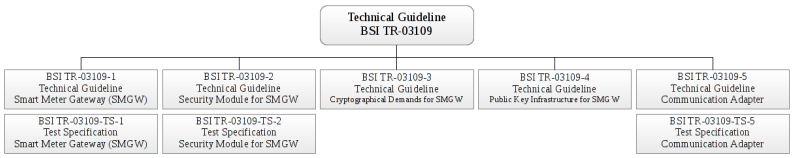
\includegraphics[width=1\textwidth]{images/BSI-TR-03109.png}
  \caption[Technical Guideline 03109 Overview]{All documents from \gls{BSI} that are subdivided under the Technical Guideline 03109 \cite{Anna}.}
  \label{fig:TG03109}
\end{figure}
\\%noch schreiben von welcher technical guideline
\\
\textbf{Stakeholder Model in the German Smart Grid}
\label{subsec:stakeholder_model}
\\
\\
The \gls{TR-03109} describes all stakeholders that participate in a power system. The most important stakeholders for this work are described.
\\\item Consumer: \\
The consumer is the person who uses electrical energy, gas, water
or heat. In addition, the consumer is the owner of the measurements processed and stored in the \gls{SMGW}. In order to interact with the \gls{SMGW}, the consumer uses a communication device. All necessary data can be retrieved and displayed through it.\\
\item SMGW administrator:\\
A Smart Meter Gateway Administrator \gls{GWA} a trusted entity and each \gls{SMGW} is assigned a \gls{GWA}. The \gls{GWA} handles the configuration, monitoring and control of \gls{SMGW}s and it is even possible to perform updates of \gls{SMGW}s via the \gls{GWA}.\\
\item Authorized external entities:\\
External market participants \gls{EMT} are all other authorized participants in the energy network that can establish a communication connection with the \gls{SMGW}. These include electricity providers. The \gls{SMGW} ignores all other communication requests that do not come from the \gls{GWA} or \gls{EMT}s in order to prevent attacks.\\
\end{enumerate}
There are several other actors such as Controllable Local Systems, service technicians and meters. However, these actors do not play a major role in the protocol that is proposed here. In Figure \ref{fig:E-Grid} is a exemplary power grid shown with the Stakeholder in the Smart Grid. Every \gls{SMGW} is connected to one \gls{GWA}, which configurates the communication profile of the \gls{SMGW}. When pseudonymization is activated, the information is not sent directly to the electricity provider, but first to the \gls{GWA}. Afterwards, the \gls{GWA} forwards the data to its electricity provider.
\begin{figure}[tbp]
  \centering
  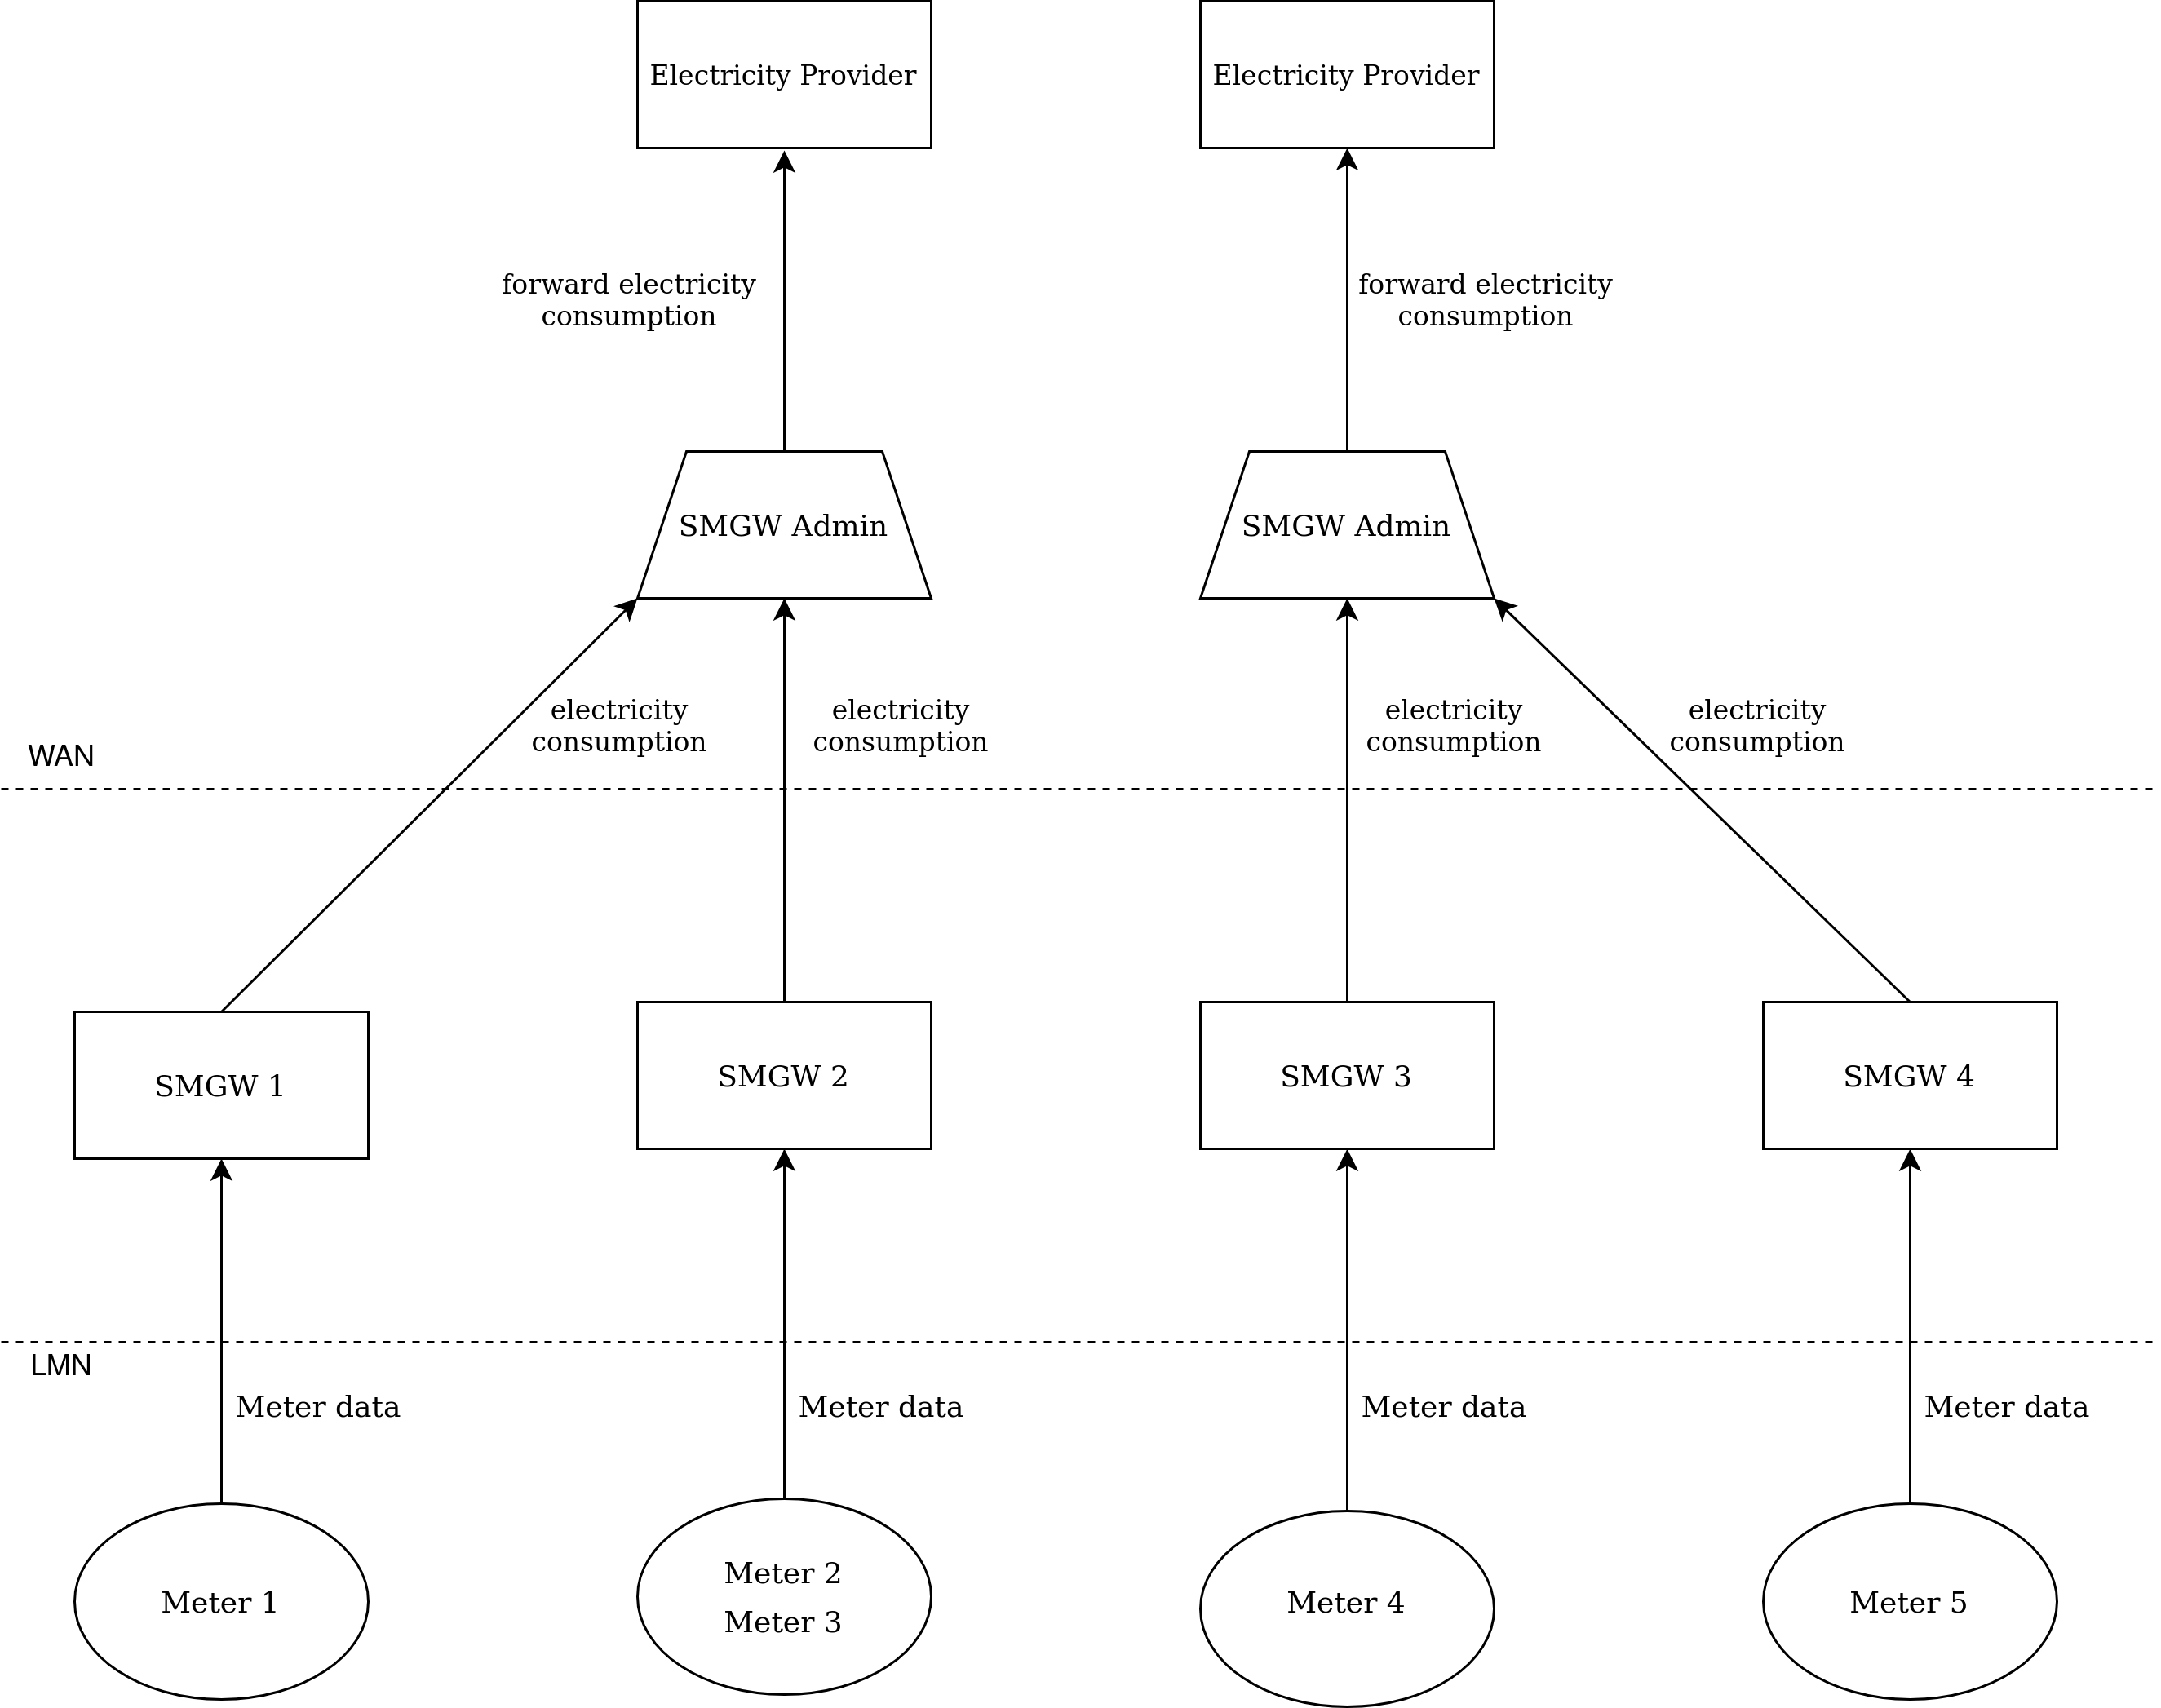
\includegraphics[width=1\textwidth]{images/grid_structure_update3.png}
  \caption[Exemplary Electricity Grid]{An exemplary electricity grid in the TG-03109 with the stakeholders.}
  \label{fig:E-Grid}
\end{figure}
\subsection{Interfaces and functions of the Smart Meter Gateway}
\begin{figure}[tbp]
  \centering
  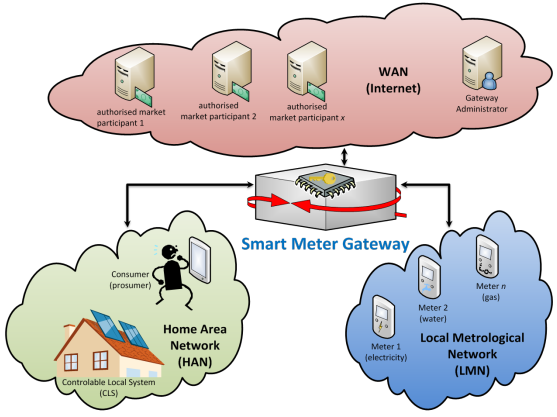
\includegraphics[width=0.7\textwidth]{images/interfaces_eng.png}
  \caption[Smart Meter Gateway Interfaces]{An overview of all interfaces and possible stakeholders that can communicate with SMGW \cite{Anna}.}
  \label{fig:Smart_Meter_Interfaces}
\end{figure}
A smart meter or as described in the \gls{TR-03109} a smart meter gateway \gls{SMGW} must provide three different physical interfaces as shown in \ref{fig:Smart_Meter_Interfaces}.
\begin{enumerate}
\item Local Metrological Network \gls{LMN}:\\
The \gls{LMN} is the communication interface in which communication takes place with the connected meters for energy and material quantities (electricity, gas). An \gls{SMGW} can communicate with one meter from one end user or with several meters from different end users. In practice, however, one \gls{SMGW} is often responsible for one meter. The measured values are sent from the meters via the \gls{LMN} to the \gls{SMGW} and stored there.
\item Wide Area Network \gls{WAN}:\\
The \gls{WAN} is the only communication interface with which the \gls{SMGW} can communicate with \gls{EMT}s or \gls{GWA}s over the Internet. If a request is made to the \gls{SMGW} that was not sent by these authorized participants, then the request is discarded and ignored.
\item Home Area Network \gls{HAN}:\\
In \gls{HAN}, an \gls{SMGW} interacts with Controllable Local Systems (e.g., photovoltaic systems). In addition, users and service technicians can use the \gls{HAN} interface to display information about power consumption through functions offered by the \gls{SMGW}.
\end{enumerate}
\begin{figure}[tbp]
  \centering
  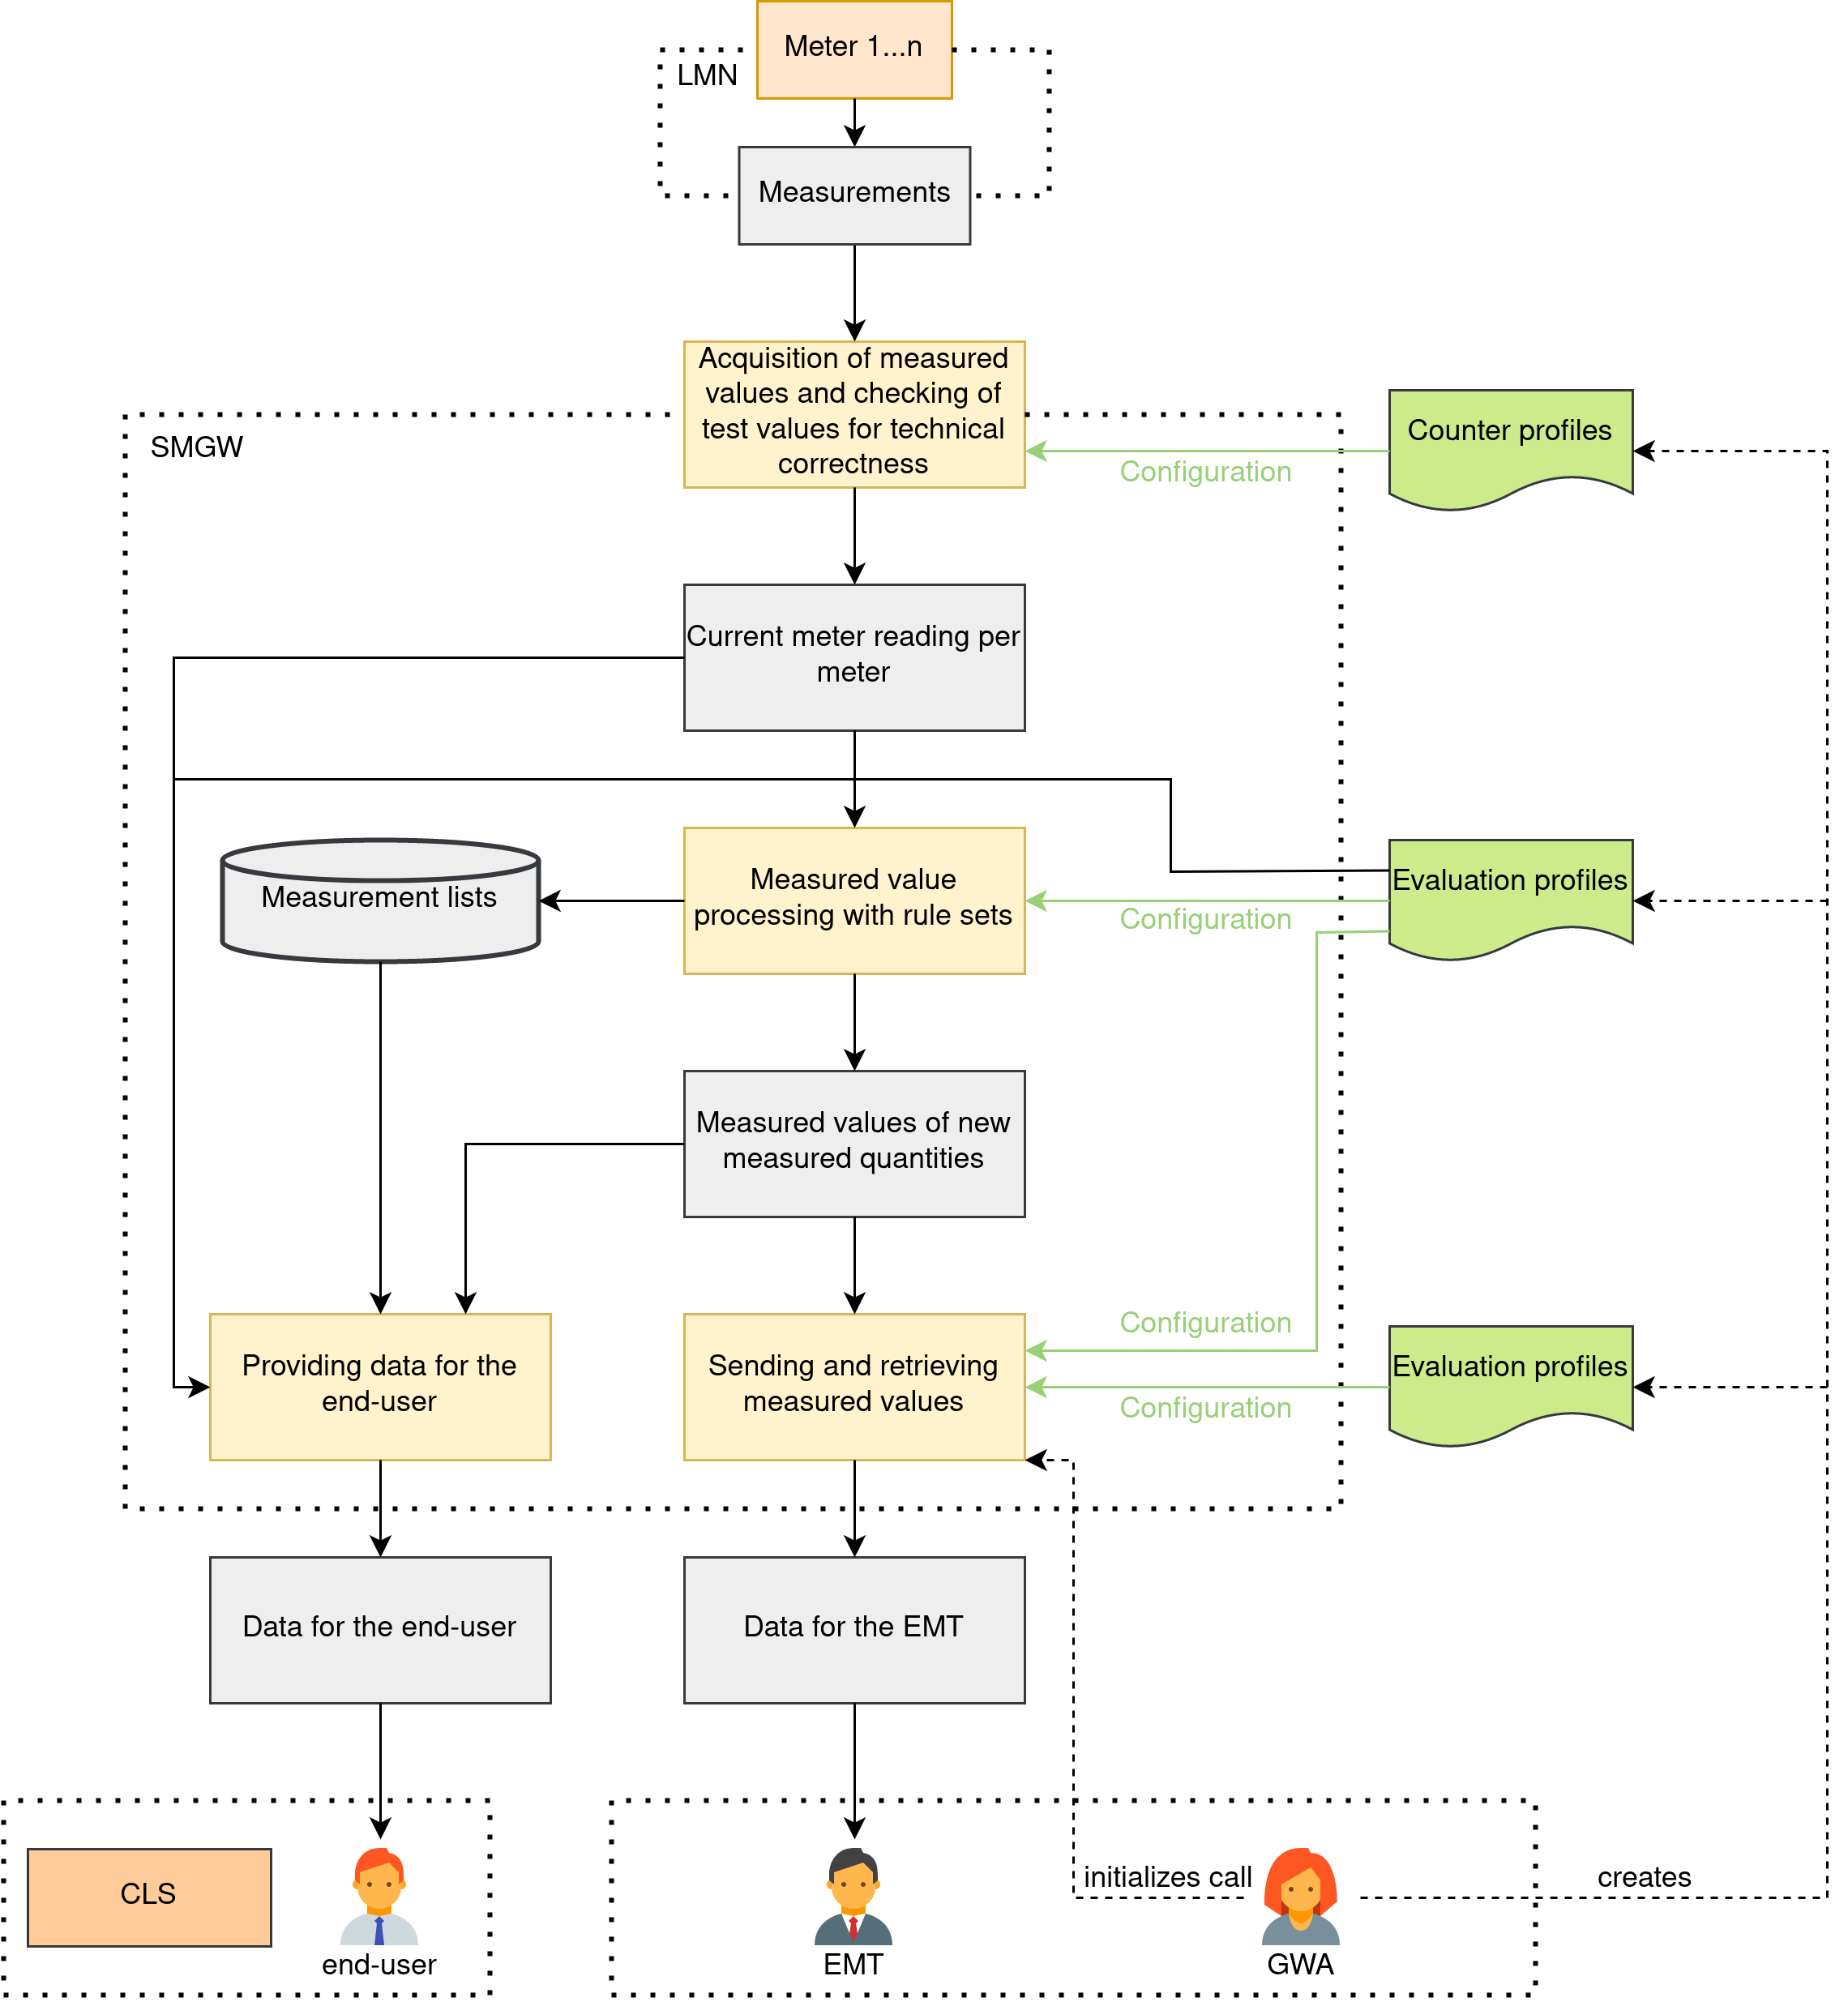
\includegraphics[width=1\textwidth]{images/MessverarbeitungEnglish2.png}
  \caption[Measured Value Processing in a SMGW]{An overview of the measured value processing within the \gls{SMGW} with configuration profiles from the GWA.}
  \label{fig:value_processing}
\end{figure}
\textbf{Functionality of the Smart Meter Gateway}
\\
\\
First, the task of \gls{SMGW} is to store the measurements sent by meters from the \gls{LMN}. Then, the readings are processed in the \gls{SMGW} and sent to the authorized \gls{EMT}s in the \gls{WAN} after processing. An \gls{SMGW} must also perform the tasks of a firewall and separate the three interfaces. As a result it is impossible for an \gls{EMT} or \gls{GWA} to make requests to devices located in the \gls{HAN} or \gls{LMN}, even if it is allowed to interact with the \gls{SMGW} over the \gls{WAN}. The processing of data from the \gls{SMGW} is shown in Fig \ref{fig:value_processing}. Since the \gls{WAN} interface is the most important interface for this work, it will be discussed in more detail.\\
\\
\textbf{Functions of the SMGW in the WAN}
\\
\\
The tasks performed by the \gls{WAN} have already been explained in the paragraph above. Now the functions and security mechanisms offered by the \gls{SMGW} to guarantee secure interaction on the \gls{WAN} will be described.
\begin{enumerate}
\item Transmission of measured values based on evaluation and \gls{WAN} communication profiles:\\
Communication profiles of \gls{GWA}s are stored in \gls{SMGW}. The communication profiles determine how the data is processed in the \gls{SMGW} and forwarded to \gls{EMT}s.

\item Pseudonymization:\\
Data that is not relevant for billing must be pseudonomized for data protection reasons. For this purpose, the unique identification number that each \gls{SMGW} has is replaced by a pseudonym. Subsequently, the information is not sent directly to an \gls{EMT}, but is forwarded to the \gls{EMT} via the \gls{GWA}. This additionally protects the identity of the sending \gls{SMGW}.%vllt als extra part machen. was unten kommt.
Even if peusodonymization does not allow an \gls{SMGW} to be directly assigned, the described attack in \ref{subsec:NILM_sec} and the resulting behavioral analysis is still possible. Since no other security mechanisms are available from the \gls{SMGW}, the question must be asked whether pseudonymization as proposed in the \gls{TR-03109} is sufficient.

\item Time synchronization:\\
In order for the cost electricity consumption to be calculated correctly, it is essential that the \gls{SMGW} have an accurate time. For this purpose, the system time of the \gls{SMGW} is synchronized with the time server of the \gls{GWA} at regular intervals.

\item Wake-Up Service:\\
A \gls{GWA} is able to force a communication link with the \gls{SMGW}. This is done via a data packet signed by the \gls{GWA}. The \gls{SMGW} then establishes a fixed preconfigured communication connection to the \gls{GWA}. This enables the \gls{GWA} to execute administration commands on the SGMW. 
\end{enumerate}
\\
\\
\textbf{Stakeholder Motives}
\\
\\
It has already been explained which participants in the power grid interact with each other. %Now in particular it will be discussed which motives the different participants have and which malicious motives can be pursued by the participants or by attackers.
Below the particular motives of the participants are discussed and which malicious intentions can be pursued by the participants.
\\
\\
\textbf{Customer's Motives}
\\
\\
For the costumer, all the security goals defined above are important. But by far the most important is the security goal of anonymity through the smart meter. Possible attacks on the electricity consumption penetrate deeply into the private sphere of each customer. Therefore, no conclusions may be drawn from the electricity consumption of a customer.\\
\begin{samepage}\enlargethispage{\baselineskip}On the other hand, unethical customers may try to steal electricity to save energy costs. The smart meter is located in or on the customer's house. An unethical customer could attempt to tamper directly with the smart meter's hardware or software. The attempts could look like this, a Costumer could try to reduce the recorded electricity consumption at the smart meter or the smart meter could be manipulated to measure less electricity when electricity prices are high and more electricity when electricity \nopagebreak prices~are~low~\cite{lemay2007unified}.\nopagebreak
\end{samepage}
\\
\\
\textbf{Electricity Provider's Motives}
\\
\\
For the electricity provider, the authenticity of the billing is the most important security objective because from its point of view, the customer is not trustworthy in the calculation of the bill. In addition, the customer has access to the smart meter at almost any time in an environment trusted by the customer. Unlike analog meters, smart meters cannot be mechanically attacked. But if a customer manages to change the software of the smart meter, the billing can be manipulated at the same time. On the other hand, the electricity provider can also be an overly intrusive electricity provider. In the paragraph \ref{subsec:NILM_sec} it was explained how a behavioral analysis can be created from the electricity consumption. This sensitive information could be used to gain an additional source of income. In \cite{quinn2009privacy} it was listed which questions could be answered by a \gls{NILM} analysis. Quote: "On what days and during what times do you watch TV? How much home time do you spend in front of your computer?" or "Are any of the appliances in your household failing or operating below optimal efficiency? Do you own (and so presumably like) lots of gadgets?". Advertising companies would certainly pay money for this kind of information in order to be able to advertise more accurately. For this reason, it is presumed that the typical electricity provider is considered an honest-but-curious adversary. But in the proposed network protocol in Chapter 3, the electricity provider gets administrative rights to maintain the network. For this reason, the electricity provider is always assumed to be malicious to be able to protect the network from the potential strongest attacker. But in the proposed protocol in Chapter 3, the electricity provider partly performs administrative tasks for the network protocol. For this reason, an additional aim is to ensure that even stronger attacks can be prevented if the electricity provider takes on the role of the much more dangerous malicious adversary \cite{lemay2007unified}.

\subsection{Security Objectives}

The smart meter attempts to achieve the three security objectives of confidentiality, integrity and availability. The three security goals are often summarized as CIA. Another important security goal for this work is anonymity. The four definitions are essential for the understanding of this work. Therefore, the terms are explained below.
\begin{enumerate}
\item Confidentiality: \\
It is not possible for an unauthorized party to gain information about the content of the data sent.
\item Integrity:\\
It is not possible for an unauthorized party to modify the content of data without data without this being noticed.
\item Availability: \\
It is not possible for an unauthorized party to interfere with the functionality of a service.
\end{enumerate}
In the application field of this thesis, anonymity is considered as follows:
\begin{enumerate}[resume]
\item Anonymity:\\
%A user is anonymous if the behavior of the user in his messages towards a recipient remains secret.
A user is anonymous if the behavior of the user sent in a message to its recipient remains secret.
%The transmitted data shouldn’t allow the receiver to recognize personal behavior.
\end{enumerate}
In the \ref{sec:design} chapter, the design of the network protocol is presented, which fulfills the mentioned security objectives and thus protects the privacy of the customer from the electricity provider or an attacker. For an attacker his main goal is to try to bypass the security objectives to obtain additional information about the customer.
\subsection{Attacks on the Smart Grid}
\label{subsec:attacks}
In Germany, the smart grid is one of the critical infrastructures. This means that the failure of the smart grid could lead to a significant compromise of public safety or other serious consequences. Such systems are threatened by all sorts of attackers. The two most common attacks that are relevant to the work are explained below.
\\
\\
\textbf{Eavesdropping}
\\
\\
Eavesdropping may be the weakest type of attack and it is often used by a passive attacker or by an active attacker as a preparation for a larger attack. Successful eavesdropping on the communications of the smart meter could be useful to e.g. intruders. However, curious neighbors might also have an interest in the behavior inside the house. Turning on/off lights implies that someone is at home or leaving the house. Therefore, eavesdropping on electricity consumption could provide information about when is a suitable time to break in. To prevent eavesdropping, smart meter communication is encrypted to maintain confidentiality. Cryptographic algorithms such as AES are widely used today and have been analyzed for weaknesses over the years by a number of researchers. Hence, a successful attack on encrypted data to extract information is extremely unlikely \cite{lemay2007unified}.
\\
\\
\textbf{Active Attackers}
\\
\\
The objective of active attackers may not necessarily be to analyze a user's electricity consumption. They may want to disable availability through e.g. denial of service attacks. These attacks could leave major damage to the power grid and are definitely a realistic threat. But this thesis focuses on smart meters and the anonymization of electricity consumption. That's why it is assumed that the active attacker does not carry out system-wide attacks on the power grid. Rather, it is assumed that the attacker attempts to take control in the proposed DC network. Among other things, it is assumed that the attacker has the theoretical ability to take over one or more \gls{SMGW} and send messages through the \gls{SMGW}. In addition, if the attacker has taken over an \gls{SMGW}, it can perform all operations that are possible through the proposed DC network.\\In the next section, the conceptual solution of the DC network is proposed and how the DC network could be implemented in the \gls{TR-03109} of the \gls{BSI}. It also describes which attacks on the DC network are possible with the defined attacker model.

\clearpage

%%% Local Variables:
%%% TeX-master: "diplom"
%%% End:
